% This file was created by matlab2tikz.
%
%The latest updates can be retrieved from
%  http://www.mathworks.com/matlabcentral/fileexchange/22022-matlab2tikz-matlab2tikz
%where you can also make suggestions and rate matlab2tikz.
%
\definecolor{mycolor1}{rgb}{0.00000,0.44700,0.74100}%
\definecolor{mycolor2}{rgb}{0.85000,0.32500,0.09800}%
\definecolor{mycolor3}{rgb}{0.92900,0.69400,0.12500}%
\definecolor{mycolor4}{rgb}{0.49400,0.18400,0.55600}%
\definecolor{mycolor5}{rgb}{0.46600,0.67400,0.18800}%
%
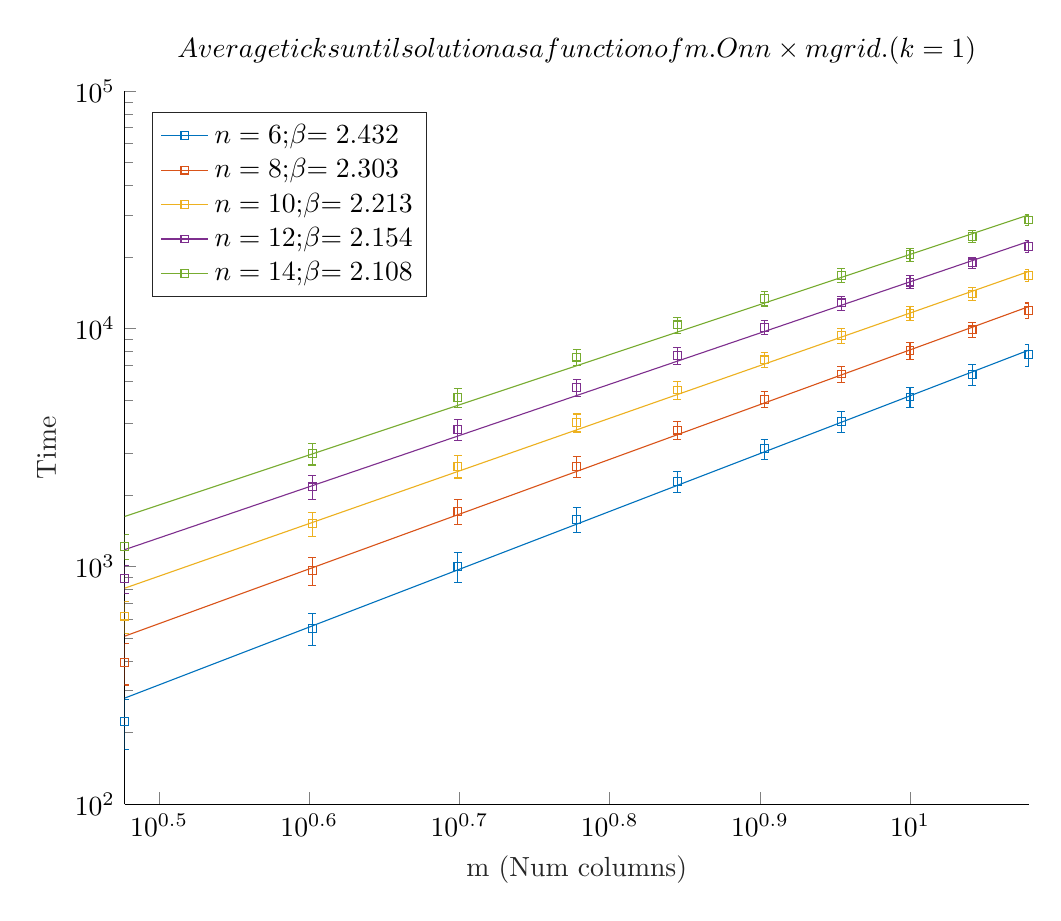
\begin{tikzpicture}

\begin{axis}[%
width=4.521in,
height=3.566in,
at={(0.758in,0.481in)},
scale only axis,
xmode=log,
xmin=3,
xmax=12,
xminorticks=true,
xlabel style={font=\color{white!15!black}},
xlabel={m (Num columns)},
ymode=log,
ymin=100,
ymax=100000,
yminorticks=true,
ylabel style={font=\color{white!15!black}},
ylabel={Time},
axis background/.style={fill=white},
title style={font=\bfseries},
title={$\text{Average ticks until solution as a function of m. On n }\times\text{ m grid. (k = 1)}$},
axis x line*=bottom,
axis y line*=left,
legend style={at={(0.03,0.97)}, anchor=north west, legend cell align=left, align=left, draw=white!15!black}
]
\addplot [color=mycolor1, draw=none, mark size=1.4pt, mark=square, mark options={solid, mycolor1}]
 plot [error bars/.cd, y dir = both, y explicit]
 table[row sep=crcr, y error plus index=2, y error minus index=3]{%
3	222.472	52.1411412727652	52.1411412727652\\
4	549.578	85.2898389566924	85.2898389566924\\
5	1001.042	143.90067074925	143.90067074925\\
6	1575.098	190.799920375325	190.799920375325\\
7	2276.66	234.552121703453	234.552121703453\\
8	3124.486	303.367139034689	303.367139034689\\
9	4074.182	427.878961491886	427.878961491886\\
10	5159.664	504.911618591985	504.911618591985\\
11	6427.76	638.573176545654	638.573176545654\\
12	7776.634	836.379936895716	836.379936895716\\
};
\addlegendentry{$\text{n =  6; }\beta\text{ = 2.432}$}

\addplot [color=mycolor1, forget plot]
  table[row sep=crcr]{%
3	279.270997066568\\
4	562.107745064538\\
5	967.075310854319\\
6	1506.58204940784\\
7	2191.67771442564\\
8	3032.40024006321\\
9	4037.99714828217\\
10	5217.07702934628\\
11	6577.7185135181\\
12	8127.55171657476\\
};
\addplot [color=mycolor2, draw=none, mark size=1.4pt, mark=square, mark options={solid, mycolor2}]
 plot [error bars/.cd, y dir = both, y explicit]
 table[row sep=crcr, y error plus index=2, y error minus index=3]{%
3	394.614	77.4461672495372	77.4461672495372\\
4	960.756	131.5821728062	131.5821728062\\
5	1702.446	205.730204194318	205.730204194318\\
6	2631.208	265.988044874261	265.988044874261\\
7	3744.352	326.707624397839	326.707624397839\\
8	5038.374	386.310369427296	386.310369427296\\
9	6450.922	500.260949857076	500.260949857076\\
10	8104.354	660.043759316324	660.043759316324\\
11	9883.782	726.950088615909	726.950088615909\\
12	11950.274	869.267364177932	869.267364177932\\
};
\addlegendentry{$\text{n =  8; }\beta\text{ = 2.303}$}

\addplot [color=mycolor2, forget plot]
  table[row sep=crcr]{%
3	508.817065535932\\
4	986.897314207056\\
5	1649.82322083576\\
6	2510.59614129317\\
7	3580.49161630291\\
8	4869.5312259055\\
9	6386.77691583397\\
10	8140.52847791842\\
11	10138.4632436838\\
12	12387.7389569023\\
};
\addplot [color=mycolor3, draw=none, mark size=1.4pt, mark=square, mark options={solid, mycolor3}]
 plot [error bars/.cd, y dir = both, y explicit]
 table[row sep=crcr, y error plus index=2, y error minus index=3]{%
3	618.156	94.5756033737401	94.5756033737401\\
4	1513.952	178.217295751591	178.217295751591\\
5	2637.64	283.359269039679	283.359269039679\\
6	4027.648	349.666167871454	349.666167871454\\
7	5525.28	481.03145023192	481.03145023192\\
8	7391.572	526.761973922132	526.761973922132\\
9	9337.908	650.860546074867	650.860546074867\\
10	11583.686	776.300924677609	776.300924677609\\
11	13998.248	846.538863011722	846.538863011722\\
12	16777.122	1022.34873354544	1022.34873354544\\
};
\addlegendentry{$\text{n = 10; }\beta\text{ = 2.213}$}

\addplot [color=mycolor3, forget plot]
  table[row sep=crcr]{%
3	809.727445135911\\
4	1530.66199619012\\
5	2508.30722561903\\
6	3755.26991978943\\
7	5282.28391388476\\
8	7098.74536942834\\
9	9213.04128904744\\
10	11632.7669644155\\
11	14364.8780054665\\
12	17415.8011503591\\
};
\addplot [color=mycolor4, draw=none, mark size=1.4pt, mark=square, mark options={solid, mycolor4}]
 plot [error bars/.cd, y dir = both, y explicit]
 table[row sep=crcr, y error plus index=2, y error minus index=3]{%
3	887.67	120.7673076009	120.7673076009\\
4	2160.546	243.150101434598	243.150101434598\\
5	3762.974	375.538194055397	375.538194055397\\
6	5653.65	457.710429392152	457.710429392152\\
7	7710.138	640.458765117342	640.458765117342\\
8	10132.224	720.057950952185	720.057950952185\\
9	12838.396	862.119634222202	862.119634222202\\
10	15703.31	988.774250745778	988.774250745778\\
11	18914.808	1060.86141461457	1060.86141461457\\
12	22220.482	1229.24706482006	1229.24706482006\\
};
\addlegendentry{$\text{n = 12; }\beta\text{ = 2.154}$}

\addplot [color=mycolor4, forget plot]
  table[row sep=crcr]{%
3	1176.125557538\\
4	2185.87678098589\\
5	3535.18130936197\\
6	5236.03195473815\\
7	7298.51629579146\\
8	9731.37655330012\\
9	12542.349536589\\
10	15738.3896497924\\
11	19325.8236072971\\
12	23310.462437726\\
};
\addplot [color=mycolor5, draw=none, mark size=1.4pt, mark=square, mark options={solid, mycolor5}]
 plot [error bars/.cd, y dir = both, y explicit]
 table[row sep=crcr, y error plus index=2, y error minus index=3]{%
3	1215.818	144.159469968376	144.159469968376\\
4	2978.586	308.05283914844	308.05283914844\\
5	5131.972	453.41852181826	453.41852181826\\
6	7592.148	599.742688726893	599.742688726893\\
7	10372.798	802.144363787912	802.144363787912\\
8	13382.324	922.408224643395	922.408224643395\\
9	16746.834	1127.93949547611	1127.93949547611\\
10	20494.166	1253.50613948535	1253.50613948535\\
11	24387.434	1401.67633451431	1401.67633451431\\
12	28636.5	1482.42014725447	1482.42014725447\\
};
\addlegendentry{$\text{n = 14; }\beta\text{ = 2.108}$}

\addplot [color=mycolor5, forget plot]
  table[row sep=crcr]{%
3	1621.44258504504\\
4	2973.40792511864\\
5	4759.12255728227\\
6	6989.23410974559\\
7	9672.61292980754\\
8	12816.885583309\\
9	16428.7560506459\\
10	20514.214944523\\
11	25078.6837757961\\
12	30127.1188331805\\
};
\end{axis}
\end{tikzpicture}%